\documentclass[a4paper,12pt]{book}

% Paquetes necesarios
\usepackage[utf8]{inputenc}   % Codificación de caracteres
\usepackage[spanish]{babel}   % Idioma español
\usepackage[T1]{fontenc}      % Codificación de fuentes
\usepackage{amsmath, amssymb} % Símbolos matemáticos
\usepackage{graphicx}         % Inclusión de gráficos
\usepackage{cite}             % Gestión de citas
\usepackage{hyperref}         % Enlaces y referencias
\usepackage{geometry}         % Configuración de márgenes
\usepackage{fancyhdr}         % Encabezados y pies de página
\usepackage{titlesec}         % Formato de títulos
\usepackage{booktabs}         % Tablas profesionales
\usepackage{caption}          % Personalización de leyendas
\usepackage{enumitem}         % Personalización de listas
\usepackage{float}
\usepackage{tcolorbox}
\usepackage[table]{xcolor} % Paquete para colores en tablas
\usepackage{colortbl}       % Complemento para colorear celdas específicas
\usepackage{multirow}       % Combinar celdas en tablas
\usepackage{makecell}       % Combinar celdas en tablas
\usepackage{enumitem}
\usepackage{amsmath}
\usepackage{eurosym}
\usepackage{tikz}
\usepackage{listings}
\usepackage{color}
\usepackage{float}
\usepackage{pdfpages}
\usepackage{subcaption}
\usepackage{pgffor}
\usepackage{stackengine}
\usetikzlibrary{shapes, arrows, positioning}
% Configuración de márgenes
\geometry{left=3cm, right=3cm, top=2.5cm, bottom=2.5cm}
\usetikzlibrary{calc}


% Configuración de encabezados y pies de página
% \setlength{\headheight}{14.49998pt}
\pagestyle{fancy}
\fancyhf{}
\fancyhead[L]{Universidad de Granada}
\fancyhead[L]{\nouppercase{\leftmark}}

% \fancyhead[C]{Escuela Técnica Superior de Ingenierías Informática}
\fancyhead[R]{Fundamentos de Base de Datos}
\fancyfoot[L]{\rule[0pt]{\textwidth}{0.2pt}\\Ismael Sallami Moreno}
\fancyfoot[C]{\rule[0pt]{\textwidth}{0.2pt}\\\thepage}
\fancyfoot[R]{\rule[0pt]{\textwidth}{0.2pt}\\\today}
\renewcommand{\sectionmark}[1]{\markboth{#1}{}} % Configura \leftmark para que solo muestre la sección

% \renewcommand{\ejercicio}[1]{%
%     \ifnum#1=8
%         Ejercicio 1. Primera forma.%%
%     \else\ifnum#1=9
%         Ejercicio 1. Segunda forma.%%
%     \else\ifnum#1=10
%         Ejercicio 2.%
%     \else\ifnum#1=11
%         Ejercicio 3.%
%     \else\ifnum#1=12
%         Ejercicio 4.%
%     \else\ifnum#1=13
%         Ejercicio 5. Primera forma.%
%     \else\ifnum#1=14
%         Ejercicio 5. Segunda forma.%
%     \else\ifnum#1=15
%         Ejercicio 6. Primera forma.%
%     \else\ifnum#1=16
%         Ejercicio 6. Segunda forma.%
%     \else\ifnum#1=17
%         Ejercicio 7.%
%     \else\ifnum#1=18
%         Ejercicio 8.%
%     \else\ifnum#1=19
%         Ejercicio 9.%
%     \else\ifnum#1=20
%         Ejercicio 10.%
%     \else\ifnum#1=21
%         Ejercicio 11.%
%     \else\ifnum#1=22
%         Ejercicio 12.%
%     \else\ifnum#1=23
%         Ejercicio 13.%
%     \else\ifnum#1=24
%         Ejercicio 14.%
%     \else\ifnum#1=25
%         Ejercicio 15.%
%     \else\ifnum#1=26
%         Ejercicio 16.%
%     \else
%         Ejercicio #1%
%     \fi\fi\fi\fi\fi\fi\fi\fi\fi\fi\fi\fi\fi\fi\fi\fi\fi\fi\fi\fi\fi\fi\fi\fi\fi\fi
% }

\newcommand{\ejercicio}[1]{%
    \ifcase#1
        % No hay caso 0
    \or % Caso 1
        % No hay caso 1
    \or % Caso 2
        % No hay caso 2
    \or % Caso 3
        % No hay caso 3
    \or % Caso 4
        % No hay caso 4
    \or % Caso 5
        % No hay caso 5
    \or % Caso 6
        % No hay caso 6
    \or % Caso 7
        % No hay caso 7
    \or % Caso 8
        Ejercicio 1. Primera forma. Formato libreta.
    \or % Caso 9
        Ejercicio 1. Segunda forma. Formato libreta.
    \or % Caso 10
        Ejercicio 2. Formato libreta.
    \or % Caso 11
        Ejercicio 3. Formato libreta.
    \or % Caso 12
        Ejercicio 4. Formato libreta.
    \or % Caso 13
        Ejercicio 5. Primera forma. Formato libreta.
    \or % Caso 14
        Ejercicio 5. Segunda forma. Formato libreta.
    \or % Caso 15
        Ejercicio 6. Primera forma. Formato libreta.
    \or % Caso 16
        Ejercicio 6. Segunda forma. Formato libreta.
    \or % Caso 17
        Ejercicio 7. Formato libreta.
    \or % Caso 18
        Ejercicio 8. Formato libreta.
    \or % Caso 19
        Ejercicio 9. Formato libreta.
    \or % Caso 20
        Ejercicio 10. Formato libreta.
    \or % Caso 21
        Ejercicio 11. Formato libreta.
    \or % Caso 22
        Ejercicio 12. Formato libreta.
    \or % Caso 23
        Ejercicio 13. Formato libreta.
    \or % Caso 24
        Ejercicio 14. Formato libreta.
    \or % Caso 25
        Ejercicio 15. Formato libreta.
    \or % Caso 26
        Ejercicio 16. Formato libreta.
    \else
        Ejercicio #1. Formato libreta.
    \fi
}




% Formato de títulos
\titleformat{\section}{\large\bfseries}{\thesection.}{0.5em}{}
\titleformat{\subsection}{\normalsize\bfseries}{\thesubsection.}{0.5em}{}

% Datos del documento
\title{\textbf{Temario Inteligencia Artificial}}
\author{
    Ismael Sallami Moreno \\
    \texttt{ism350zsallami@correo.ugr.es}
}
\date{
    \vspace{1cm}
    \begin{tabular}{rl}
        \textbf{Asignatura:} & Fundamentos de Base de Datos \\
        \textbf{Tema:} & Teoría \\
        \textbf{Fecha:} & \today
    \end{tabular}
}
\renewcommand{\b}[1]{\textbf{#1}}

\begin{document}

% Portada
\begin{titlepage}
    \begin{center}
        % \vspace*{1cm}
        
        % \Huge
        % \textbf{Práctica Contabilidad Financiera II}
        \Huge \textbf{Prácticas Fundamentos de Bases de Datos} 
        % \vspace{0.5cm}
        % \LARGE
        % \textbf{Ismael Sallami Moreno}\\
        % \LARGE
        % \texttt{ism350zsallami@correo.ugr.es}
        % \LARGE
        % \url{https://github.com/Ismael-Sallami}
        
        % \vfill
        
        % \Large
        % \textbf{Universidad de Granada}
        
        \vspace{0.8cm}
        
        \begin{tikzpicture}[remember picture, overlay]
            \node[opacity=0.2] at (current page.center) {
\includegraphics[width=\paperwidth,height=\paperheight]{portada.jpg}};
            \node[align=center] at (current page.center) {
                
                \vspace{0.5cm}
                \LARGE \textbf{Ismael Sallami Moreno} \\
                \LARGE \texttt{ism350zsallami@correo.ugr.es} \\
                \LARGE \url{https://ismael-sallami.github.io/} \\
                \LARGE \url{https://elblogdeismael.github.io/} \\
                \vspace{2cm}
                \Large \textbf{Universidad de Granada} \\
                \vspace{0.8cm}
                % \Large \textbf{2025}
            };
        \end{tikzpicture}
        \vfill
        
        \Large
        \textbf{2025}
        
    \end{center}
\end{titlepage}
\newpage


%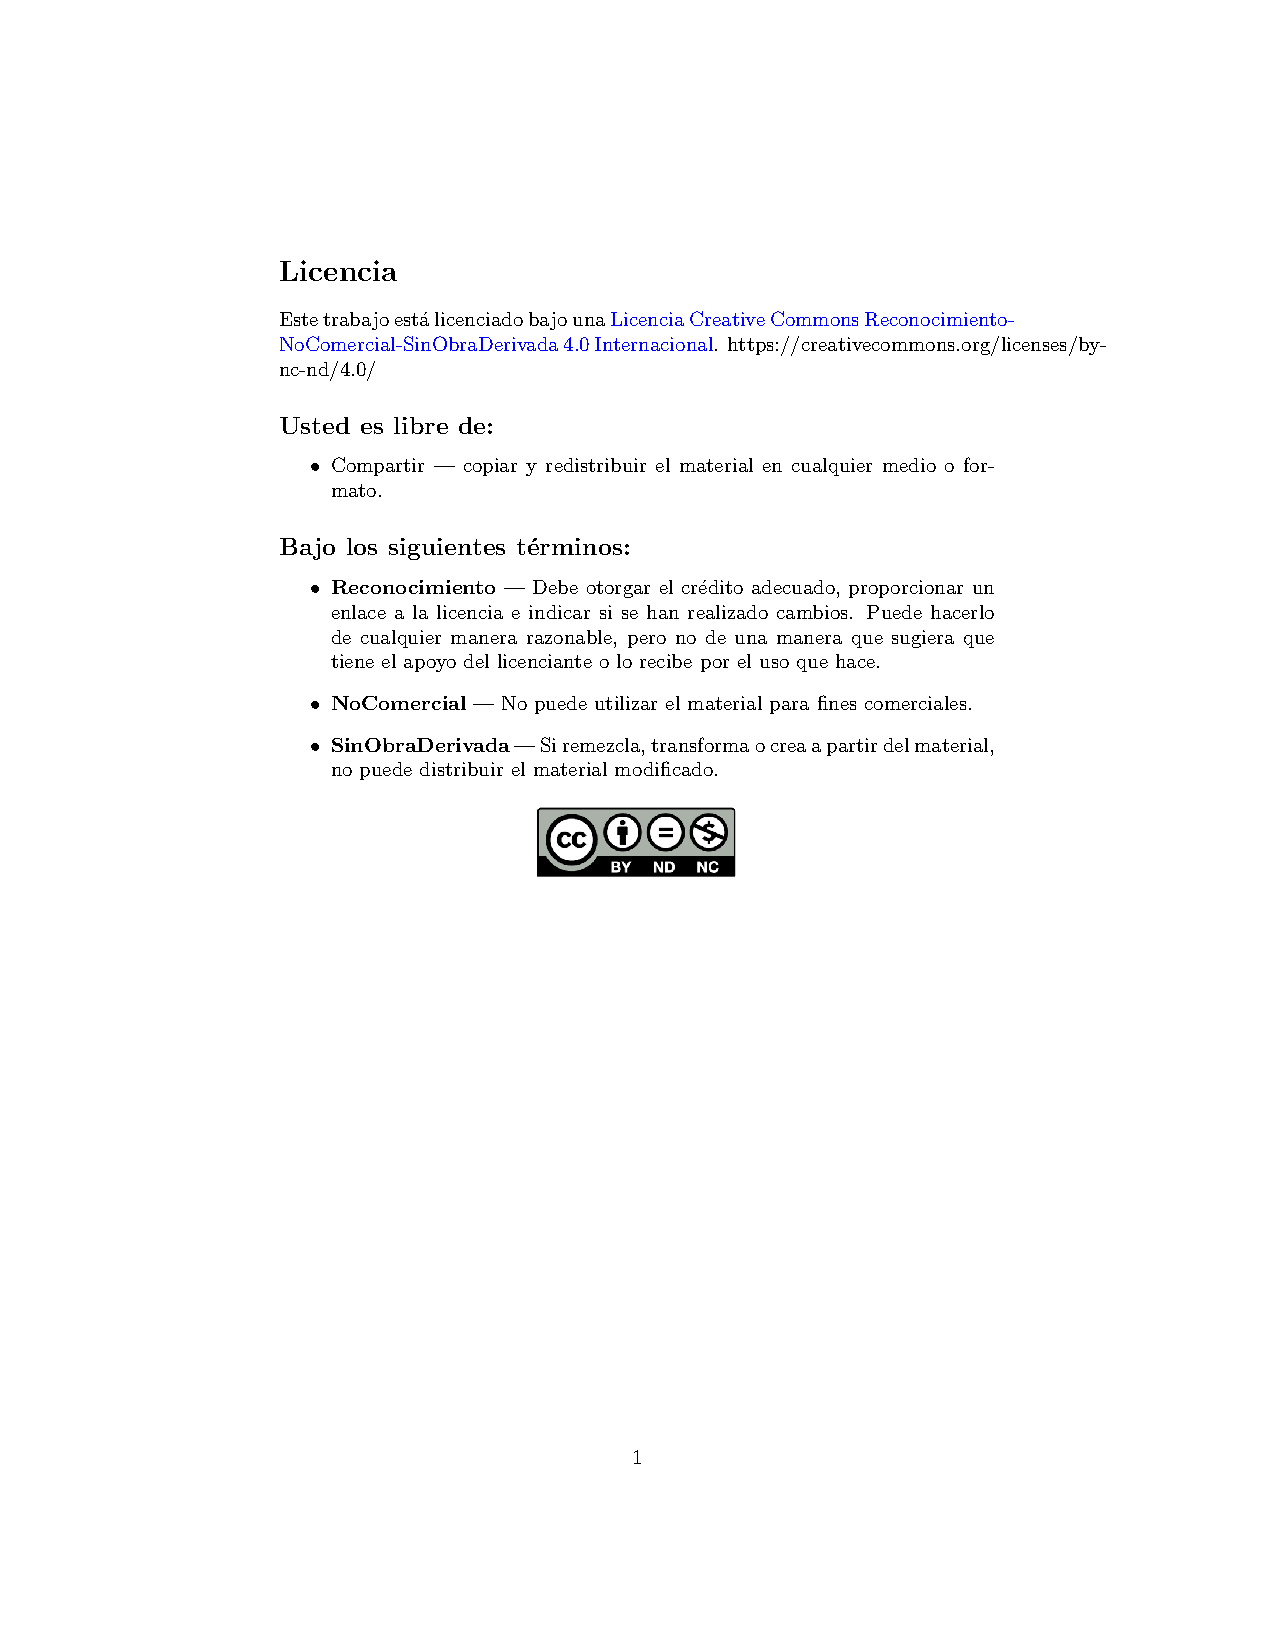
\includepdf[pages=-]{../../../../licencia.pdf}

% Tabla de contenidos
\tableofcontents
\newpage
\chapter{Modelado Conceptual}
\section{Relación de Ejercicios}
%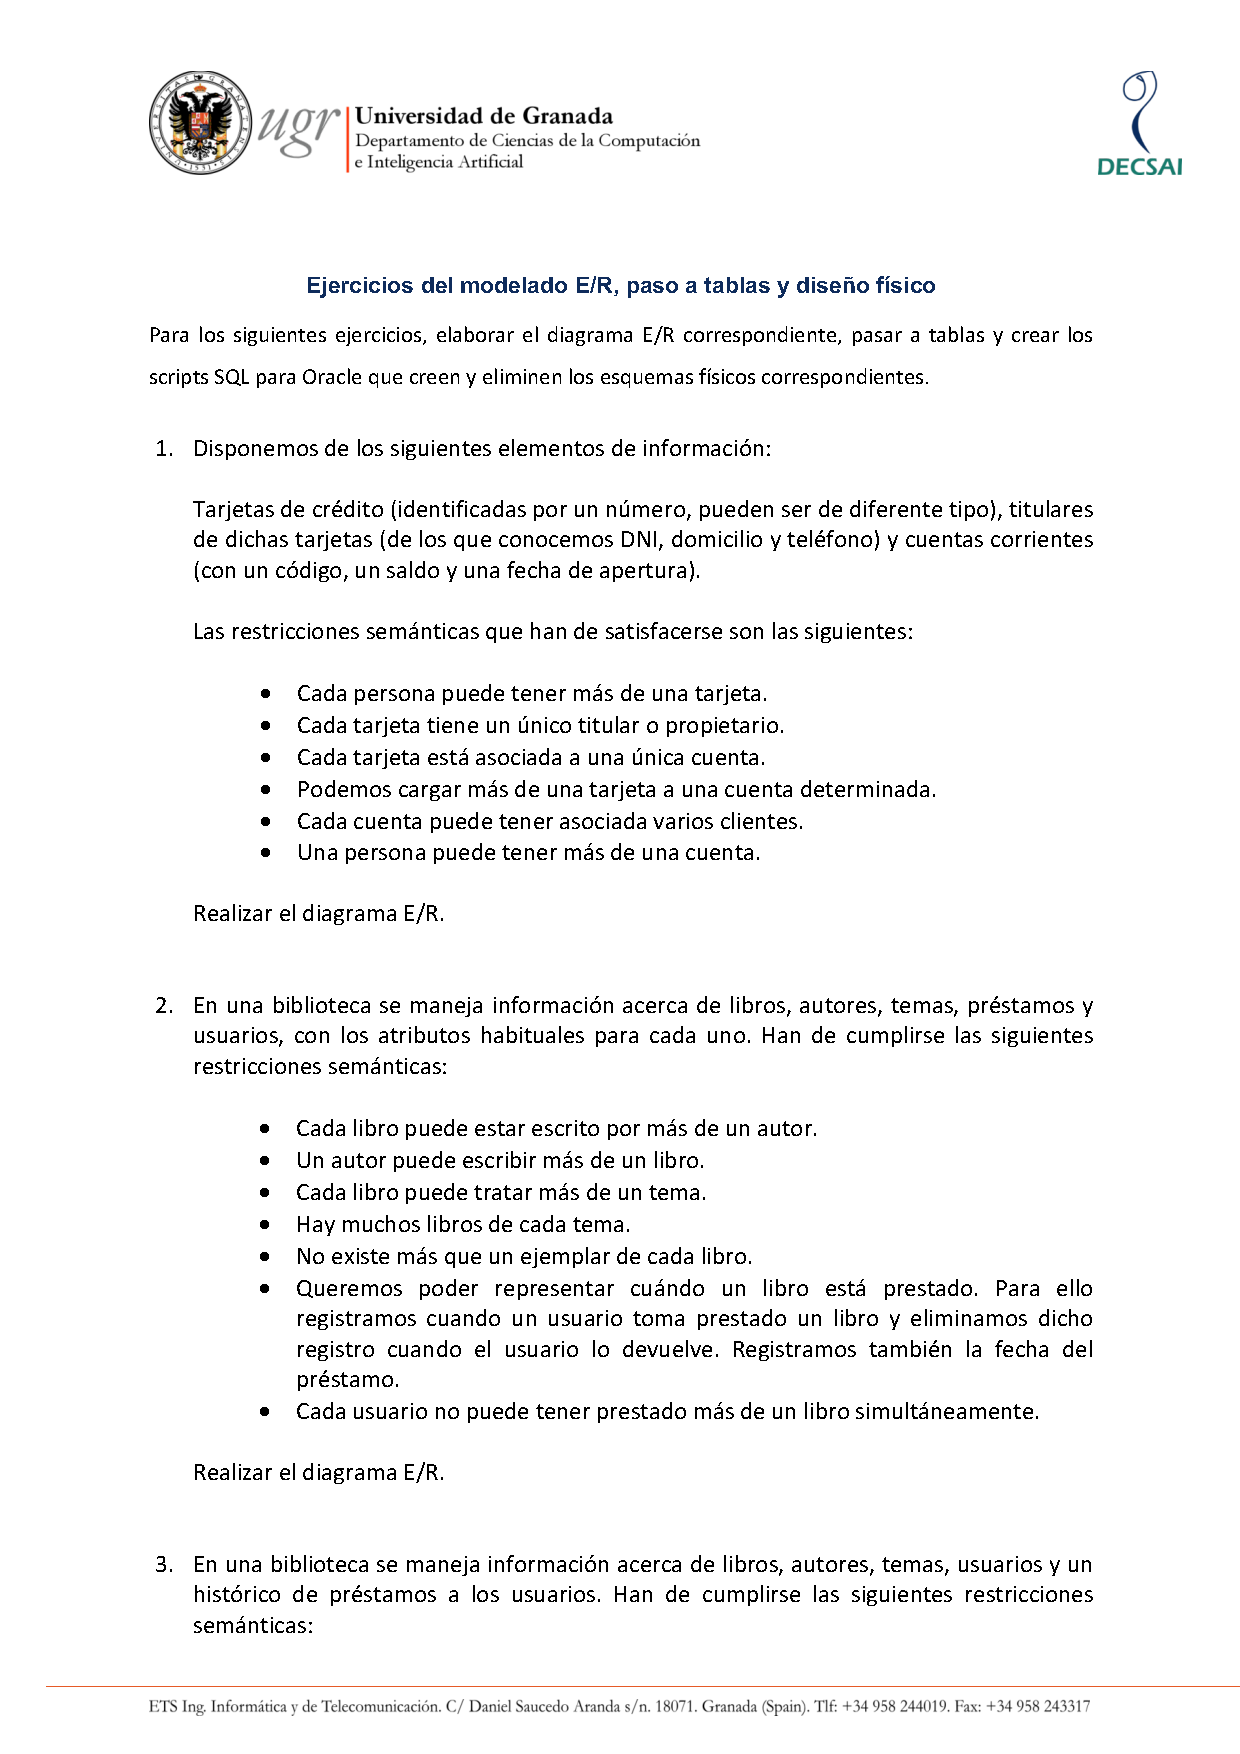
\includepdf[pages=-]{Capitulos/RelacionS1S2-SinEditar}%\includepdf[pages=-,pagecommand={\thispagestyle{fancy}}]{Capitulos/Ejercicios_FBD_S1.pdf}



% \begin{center}
%     \begin{tikzpicture}[
%         entity/.style={rectangle, draw, minimum width=3cm, minimum height=1cm},
%         relationship/.style={diamond, draw, minimum width=2cm, minimum height=1cm},
%         attribute/.style={ellipse, draw},
%         line/.style={draw, -latex},
%         singleline/.style={draw, -},
%         doubleline/.style={draw, double distance=2pt, -}
%     ]
%         % Entidades
%         \node[entity] (libro) {Libro};
%         \node[entity, right=4cm of libro] (autor) {Autor};
%         \node[entity, below=4cm of libro] (tema) {Tema};
%         \node[entity, below=4cm of autor] (usuario) {Usuario};

%         % Relaciones
%         \node[relationship, above right=1cm and 1cm of libro] (escribe) {Escribe};
%         \node[relationship, below=2cm of libro] (trata) {Trata de};
%         \node[relationship, below=2cm of escribe] (prestamo) {Préstamo};

%         % Atributos
%         \node[attribute, above left=1cm and 1cm of libro] (atributos_libro) {ISBN, Título};
%         \node[attribute, below left=1cm and 1cm of autor] (dni_autor) {DNI};
%         \node[attribute, below right=1cm and 1cm of autor] (domicilio_autor) {Domicilio};
%         \node[attribute, below left=1cm and 1cm of usuario] (dni_usuario) {DNI};
%         \node[attribute, below right=1cm and 1cm of usuario] (domicilio_usuario) {Domicilio};
%         \node[attribute, below=1cm of tema] (nombre_tema) {Nombre};

%         % Conexiones
%         \draw[doubleline] (libro) -- (escribe);
%         \draw[line] (escribe) -- (autor);
%         \draw[line] (libro) -- (trata);
%         \draw[line] (trata) -- (tema);
%         \draw[line] (libro) -- (prestamo);
%         \draw[line] (prestamo) -- (usuario);

%         \draw[line] (libro) -- (atributos_libro);
%         \draw[line] (autor) -- (dni_autor);
%         \draw[line] (autor) -- (domicilio_autor);
%         \draw[line] (usuario) -- (dni_usuario);
%         \draw[line] (usuario) -- (domicilio_usuario);
%         \draw[line] (tema) -- (nombre_tema);
%     \end{tikzpicture}
% \end{center}

\subsection*{Ejercicio 1}
\noindent Disponemos de los siguientes elementos de información: 

\begin{itemize}
    \item Tarjetas de crédito (identificadas por un número, pueden ser de diferente tipo).
    \item Titulares de dichas tarjetas (de los que conocemos DNI, domicilio y teléfono).
    \item Cuentas corrientes (con un código, un saldo y una fecha de apertura).
\end{itemize}

\noindent Las restricciones semánticas que han de satisfacerse son las siguientes: 

\begin{itemize}
    \item Cada persona puede tener más de una tarjeta.
    \item Cada tarjeta tiene un único titular o propietario.
    \item Cada tarjeta está asociada a una única cuenta.
    \item Podemos cargar más de una tarjeta a una cuenta determinada.
    \item Cada cuenta puede tener asociada varios clientes.
    \item Una persona puede tener más de una cuenta.
\end{itemize}

\noindent Realizar el diagrama E/R.

\subsubsection*{Forma 1}
\begin{figure}[H]
    \begin{center}
        \begin{tikzpicture}[
            entity/.style={rectangle, draw, minimum width=3cm, minimum height=1cm},
            relationship/.style={diamond, draw, minimum width=2cm, minimum height=1cm},
            attribute/.style={ellipse, draw},
            line/.style={draw, -latex},
            singleline/.style={draw, -},
            doubleline/.style={draw, double distance=2pt, -},
        ]
            % Entidades
            \node[entity] (tarjeta) {Tarjeta};
            \node[entity, right=4cm of tarjeta] (cc) {C.C};
            \node[entity, below=4cm of tarjeta] (persona) {Persona};

            % Relaciones
            \node[relationship, above right=1cm and 1cm of tarjeta] (asociada) {Asociada};
            \node[relationship, below right=1cm and 1cm of cc] (vinculada) {Vinculada};
            \node[relationship, below left=1cm and 1cm of tarjeta] (titular) {Titular};

            % Atributos
            \node[attribute, above left=1cm and 1cm of tarjeta] (num_tarjeta) {\textbf{Nº}};
            \node[attribute, left=1cm of tarjeta] (tipo_tarjeta) {Tipo};
            \node[attribute, above right=1cm and 1cm of cc] (codigo_cc) {\b{Código}};
            \node[attribute, right=1cm of cc] (saldo_cc) {Saldo};
            \node[attribute, below left=1cm and 0.3cm of cc] (fecha_apertura_cc) {Fecha Apertura};
            \node[attribute, below left=1cm and 1cm of persona] (dni_persona) {\b{DNI}};
            \node[attribute, below=1cm of persona] (domicilio_persona) {Domicilio};
            \node[attribute, below right=1cm and 1cm of persona] (telefono_persona) {Teléfono};

            % Conexiones
            \draw[doubleline] (tarjeta) -- (asociada);
            \draw[line] (asociada) -- (cc);
            \draw[singleline] (cc) -- (vinculada);
            \draw[singleline] (vinculada) -- (persona);
            \draw[doubleline] (tarjeta) -- (titular);
            \draw[line] (titular) -- (persona);

            \draw[line, -*] (tarjeta) -- (num_tarjeta);  % Línea con círculo relleno al final
            \draw[line, -o] (tarjeta) -- (tipo_tarjeta); % Línea con círculo vacío al final
            \draw[line, -*] (cc) -- (codigo_cc);
            \draw[line, -o] (cc) -- (saldo_cc);
            \draw[line, -o] (cc) -- (fecha_apertura_cc);
            \draw[line, -*] (persona) -- (dni_persona);
            \draw[line, -o] (persona) -- (domicilio_persona);
            \draw[line,-o] (persona) -- (telefono_persona);
        \end{tikzpicture}
    \end{center}
    \caption{Diagrama Entidad-Relación del Ejercicio 1, forma 1.}
\end{figure}

\subsubsection*{Paso a Tabla de la forma 1}

\begin{figure}[H]
    \begin{center}
        \begin{tikzpicture}
            \node (Persona) {1. Persona (\stackunder{\underline{DNI}}{CP}, Domicilio, \stackunder{Teléfono}{CC/CU})};
        
            \node (Vinculada) [below=of Persona] {2. Vinculada(\stackunder{\underline{\stackon{Código}{CE(3)}, \stackon{DNI}{CE(1)}}}{CP})};

            % \node (Titular) [right=of Persona]{3. Titular (\stackunder{\underline{\stackon{DNI}{CE(1)}}}{CP}, \stackon{Nº}{CE(3)}{CP})};

            \node (Cuenta) [right=of Persona]{3. C.C (\stackunder{
            \underline{Código}}{CP}, Saldo, Fecha Apertura)};

            \node [below=of Cuenta](Tarjeta) {4. Tarjeta (\stackunder{\underline{Nº}}{CP}, Tipo, \stackon{\stackunder{DNI}{No Nulo}}{CE(1)}, \stackon{\stackunder{Código}{No Nulo}}{CE(3)}) };

        \end{tikzpicture}
    \end{center}
    \caption{En este caso no aparece ni Titular ni Asociada, debido a que se ha hecho uso de la fusión de Tablas.}
\end{figure}








\subsubsection*{Forma 2}
% \begin{center}
%     \usetikzlibrary{calc} % Include the calc library for coordinate calculations
%     \usetikzlibrary{calc} % Include the calc library for coordinate calculations
%     \begin{tikzpicture}[
%         entity/.style={rectangle, draw, minimum width=3cm, minimum height=1cm},
%         relationship/.style={diamond, draw, minimum width=2cm, minimum height=1cm},
%         line/.style={draw, -}, % Define the 'line' style
%         doubleline/.style={draw, double distance=2pt, -}
%     ]
%         % Entidades
%         \node[entity] (tarjeta) {Tarjeta};
%         \node[entity, below left=3cm and 3cm of tarjeta] (titular) {Titular};
%         \node[entity, below right=3cm and 3cm of tarjeta] (cc) {C. Corriente};

%         % Relaciones
%         \node[relationship, below=2cm of tarjeta] (tiene) {tiene};
%         \node[relationship, below=2cm of titular] (posee) {posee};

%         % Conexiones
%         \draw[line] (tarjeta) -- (tiene);
%         \draw[line] (tiene) -- (titular);
%         \draw[doubleline] (titular) -- (posee);
%         \draw[line] (posee) -- (cc);
%     \end{tikzpicture}
% \end{center}

\begin{figure}[H]
    \begin{center}
        \begin{tikzpicture}
            [entity/.style={rectangle, draw, minimum width=3cm, minimum height=1cm},
            relationship/.style={diamond, draw, minimum width=2cm, minimum height=1cm},
            attribute/.style={ellipse, draw},
            line/.style={draw, -latex},
            singleline/.style={draw, -},
            doubleline/.style={draw, double distance=2pt, -},]
            % Nodos
            \node[draw, rectangle] (tarjeta) {Tarjeta};
            \node[draw, diamond, below=of tarjeta] (tiene) {tiene};
            \node[draw, rectangle, below left=2cm and 2cm of tiene] (titular) {Titular};
            \node[draw, rectangle, below right=2cm and 2cm of tiene] (corriente) {C. Corriente};
            \node[draw, diamond, below=of tiene] (posee) {posee};
            
            \draw[doubleline] (tarjeta) -- (tiene);
            \draw[line] (tiene) -- (posee);
            \draw[draw, -] (posee) -- (titular);
            \draw[doubleline, -] (posee) -- (corriente);
            
            % Caja de agrupación
            \draw[dashed] ($(titular.north west) + (-0.5,0.6)$) rectangle ($(corriente.south east) + (0.5,-0.6)$);
        \end{tikzpicture}
    \end{center}
    \caption{Diagrama Entidad-Relación del Ejercicio 1, forma 2 usando abstracción, los atributos son los mismo que en la forma 1.}
    
\end{figure}
\subsubsection*{Paso a tabla de la forma 2}
\begin{enumerate}
    \item Persona (\textit{DNI(CP), Domicilio, Teléfono})
    \item Posee (\textit{DNI(CE(1)), Código(CE(3))(Unión de DNI y de Código CP)})
    \item Cuenta (\textit{Código(CP), Saldo, Fecha Apertura})
    \item Tiene (\textit{número(CE(5), DNI(CE(2)), Código(CE(2))(Código y DNI CP))})
    \item Tarjeta (\textit{número(CP), tipo})
    \item Titular (\textit{DNI (CE(1)), Código(CE(1))(DNI y Código CP)})
\end{enumerate}

Podemos hacer uso de la fusión, por lo que Tarjeta y Tiene desaparecen y solo nos queda una tabla:

\begin{itemize}
    \item[7. ] Tarjeta-Tiene(\textit{número(CP), tipo, DNI, Código(DNI y Código CE(Titular))})
\end{itemize}

\newpage

\subsection*{Ejercicio 2}

\noindent En una biblioteca se maneja información acerca de libros, autores, temas, préstamos y 
usuarios, con los atributos habituales para cada uno. Han de cumplirse las siguientes 
restricciones semánticas: 
 
\begin{itemize}
    \item Cada libro puede estar escrito por más de un autor.
    \item Un autor puede escribir más de un libro.
    \item Cada libro puede tratar más de un tema.
    \item Hay muchos libros de cada tema.
    \item No existe más que un ejemplar de cada libro.
    \item Queremos poder representar cuándo un libro está prestado. Para ello registramos cuándo un usuario toma prestado un libro y eliminamos dicho registro cuando el usuario lo devuelve. Registramos también la fecha del préstamo.
    \item Cada usuario no puede tener prestado más de un libro simultáneamente.
\end{itemize}

\noindent Realizar el diagrama E/R.

\begin{figure}[H]
    \begin{center}
        \begin{tikzpicture}[
            entity/.style={rectangle, draw, minimum width=3cm, minimum height=1cm},
            relationship/.style={diamond, draw, minimum width=2cm, minimum height=1cm},
            attribute/.style={ellipse, draw},
            line/.style={draw, -latex},
            singleline/.style={draw, -},
            doubleline/.style={draw, double distance=2pt, -}
        ]
            % Entidades
            \node[entity] (libro) {Libro};
            \node[entity, right=4cm of libro] (autor) {Autor};
            \node[entity, below=6cm of libro] (tema) {Tema};
            \node[entity, below=4cm of autor] (usuario) {Usuario};
    
            % Relaciones
            \node[relationship, above right=1cm and 1cm of libro] (escribe) {Escribe};
            \node[relationship, below=2cm of libro] (trata) {Trata de};
            \node[relationship, below=2cm of escribe] (prestamo) {Préstamo};
    
            % Atributos
            \node[attribute, above left=1cm and 1cm of libro] (isbn) {ISBN};
            \node[attribute, above=1cm and 1cm of libro] (titulo) {Título};
            \node[attribute, above=1cm and 1cm of autor] (dni_autor) {DNI};
            \node[attribute, above right=1cm and 1cm of autor] (domicilio_autor) {Domicilio};
            \node[attribute, below left=1cm and 1cm of usuario] (dni_usuario) {DNI};
            \node[attribute, below right=1cm and 1cm of usuario] (domicilio_usuario) {Domicilio};
            \node[attribute, below=1cm of tema] (nombre_tema) {Nombre};
            \node[attribute, below=1cm of prestamo] (fecha) {Fecha};
    
            % Conexiones
            \draw[doubleline] (libro) -- (escribe);
            \draw[singleline] (escribe) -- (autor);
            \draw[doubleline] (libro) -- (trata);
            \draw[singleline] (trata) -- (tema);
            %\draw[singleline] (libro) -- (prestamo);
            \draw[line] (prestamo) -- (libro);
            \draw[line] (prestamo) -- (usuario);
    
            \draw[line, -*] (libro) -- (isbn);
            \draw[line, -o] (libro) -- (titulo);
            \draw[line, -*] (autor) -- (dni_autor);
            \draw[line, -o] (autor) -- (domicilio_autor);
            \draw[line, -*] (usuario) -- (dni_usuario);
            \draw[line, -o] (usuario) -- (domicilio_usuario);
            \draw[line, -*] (tema) -- (nombre_tema);
            \draw[dashed, -o] (prestamo) -- (fecha);
        \end{tikzpicture}
    \end{center}
    \caption{Diagrama Entidad-Relación del Ejercicio 2. Versión Optimizada usando el atribudo de }
\end{figure}

\subsubsection*{Paso a tabla del ejercicio 2}

\begin{enumerate}
    \item Libro (ISBN(CP), título, ...)
    \item Escribe (ISBN(CE(1)), DNI(CE(3))(ISBN y DNI CP))
    \item Autor (DNI(CP), domicilio, ...)
    \item Préstamo (ISBN(CE(1)), fecha, DNI(CE(3)), (ISBN y fecha CP)(fecha y DNI CC))
    \item Trata de (ISBN(CE(1)), Nombre(CE(6))(ISBN y Nombre CP))
    \item Tema (Nombre(CP))
    \item Usuario (DNI (CP), Nombre)
\end{enumerate}

\subsubsection*{Versión optimizada del Ejercicio 2}
\begin{figure}[H]
    \begin{center}
        \begin{tikzpicture}[
            entity/.style={rectangle, draw, minimum width=3cm, minimum height=1cm},
            relationship/.style={diamond, draw, minimum width=2cm, minimum height=1cm},
            attribute/.style={ellipse, draw},
            line/.style={draw, -latex},
            singleline/.style={draw, -},
            doubleline/.style={draw, double distance=2pt, -}, 
        ]
            % Entidades
            \node[entity] (libro) {Libro};
            \node[entity, right=4cm of libro] (autor) {Autor};
            \node[entity, below=6cm of libro] (tema) {Tema};
            \node[entity, below=4cm of autor] (usuario) {Usuario};
    
            % Relaciones
            \node[relationship, above right=1cm and 1cm of libro] (escribe) {Escribe};
            \node[relationship, below=2cm of libro] (trata) {Trata de};
            \node[relationship, below=2cm of escribe] (prestamo) {Préstamo};
    
            % Atributos
            \node[attribute, above left=1cm and 1cm of libro] (isbn) {ISBN};
            \node[attribute, above=1cm and 1cm of libro] (titulo) {Título};
            \node[attribute, above=1cm and 1cm of autor] (dni_autor) {DNI};
            \node[attribute, above right=1cm and 1cm of autor] (domicilio_autor) {Domicilio};
            \node[attribute, below left=1cm and 1cm of usuario] (dni_usuario) {DNI};
            \node[attribute, below right=1cm and 1cm of usuario] (domicilio_usuario) {Domicilio};
            \node[attribute, below=1cm of tema] (nombre_tema) {Nombre};
            \node[attribute, below=1cm of prestamo] (fecha) {Fecha};
    
            % Conexiones
            \draw[doubleline] (libro) -- (escribe);
            \draw[singleline] (escribe) -- (autor);
            \draw[doubleline] (libro) -- (trata);
            \draw[singleline] (trata) -- (tema);
            %\draw[singleline] (libro) -- (prestamo);
            \draw[line] (prestamo) -- (libro);
            \draw[line] (prestamo) -- (usuario);
    
            \draw[line, -*] (libro) -- (isbn);
            \draw[line, -o] (libro) -- (titulo);
            \draw[line, -*] (autor) -- (dni_autor);
            \draw[line, -o] (autor) -- (domicilio_autor);
            \draw[line, -*] (usuario) -- (dni_usuario);
            \draw[line, -o] (usuario) -- (domicilio_usuario);
            \draw[line, -*] (tema) -- (nombre_tema);
            \draw[dashed, -*] (prestamo) -- (fecha);
        \end{tikzpicture}
    \end{center}
    \caption{Diagrama Entidad-Relación del Ejercicio 2. Versión Optimizada usando el atribudo de }
\end{figure}

En base a esta versión optimizada, podemos fusionar Libro y Préstamo, de manera que deberíamos de elimnar ambas y añadir:
\begin{itemize}
    \item[8. ] Libro-Préstamo(\textit{ISBN(CP), Título, DNI(CE Usuario y CU),fecha})
\end{itemize}


\newpage

\subsection*{Ejercicio 3}

\noindent En una biblioteca se maneja información acerca de libros, autores, temas, usuarios y un 
histórico de préstamos a los usuarios. Han de cumplirse las siguientes restricciones 
semánticas: 

\begin{itemize}
    \item Cada libro puede estar escrito por más de un autor.
    \item Un autor puede escribir más de un libro.
    \item Existen varios ejemplares de cada libro.
    \item Cada libro trata un único tema.
    \item Hay muchos libros de cada tema.
    \item En el histórico de préstamos se registra una entrada de préstamo por cada día 
    que permanece prestada una copia.
    \item Una misma copia de un libro no puede estar prestada a varios usuarios el 
    mismo día.
    \item Un usuario puede tener prestados varios ejemplares al mismo tiempo.
\end{itemize}

\noindent Se pide: 

\begin{enumerate}[label=\alph*)]
    \item Realizar el diagrama E/R.
    \item ¿Cómo habría que modificar el esquema anterior si estableciéramos la 
    restricción de que un usuario no puede tener prestados más de un ejemplar el 
    mismo día?
\end{enumerate}

\begin{figure}[H]
    \begin{center}
        \begin{tikzpicture}[
            entity/.style={rectangle, draw, minimum width=3cm, minimum height=1cm},
            relationship/.style={diamond, draw, minimum width=2cm, minimum height=1cm},
            attribute/.style={ellipse, draw},
            line/.style={draw, -latex},
            singleline/.style={draw, -},
            doubleline/.style={draw, double distance=2pt, -}, 
        ]
            % Entidades
            \node[entity] (libro) {Libro};
            \node[entity, right=4cm of libro] (autor) {Autor};
            \node[entity, below=6cm of libro] (tema) {Tema};
            \node[entity, below=4cm of autor] (usuario) {Usuario};
            \node[entity, double distance=2pt, below right=2cm of libro, draw=black, line width=0.5mm] (ejemplares) {Ejemplares};
    
            % Relaciones
            \node[relationship, above right=1cm and 1cm of libro] (escribe) {Escribe};
            \node[relationship, below=2cm of libro] (trata) {Trata de};
            \node[relationship, below=2cm of ejemplares] (prestamo) {Préstamo};
    
            % Atributos
            \node[attribute, above left=1cm and 1cm of libro] (isbn) {ISBN};
            \node[attribute, above=1cm and 1cm of libro] (titulo) {Título};
            \node[attribute, above=1cm and 1cm of autor] (dni_autor) {DNI};
            \node[attribute, above right=1cm and 1cm of autor] (domicilio_autor) {Domicilio};
            \node[attribute, below=1cm and 1cm of usuario] (dni_usuario) {DNI};
            \node[attribute, below right=1cm and 1cm of usuario] (domicilio_usuario) {Domicilio};
            \node[attribute, below=1cm of tema] (nombre_tema) {Nombre};
            \node[attribute, below=1cm of prestamo] (fecha) {Fecha};
            \node[attribute, right=1cm of ejemplares] (numero) {Número};
    
            % Conexiones
            \draw[doubleline] (libro) -- (escribe);
            \draw[singleline] (escribe) -- (autor);
            \draw[doubleline] (libro) -- (trata);
            \draw[singleline] (trata) -- (tema);
            %\draw[singleline] (libro) -- (prestamo);
            \draw[line] (prestamo) -- (ejemplares);
            \draw[line] (prestamo) -- (usuario);
    
            \draw[line, -*] (libro) -- (isbn);
            \draw[line, -o] (libro) -- (titulo);
            \draw[line, -*] (autor) -- (dni_autor);
            \draw[line, -o] (autor) -- (domicilio_autor);
            \draw[line, -*] (usuario) -- (dni_usuario);
            \draw[line, -o] (usuario) -- (domicilio_usuario);
            \draw[line, -*] (tema) -- (nombre_tema);
            \draw[dashed, -*] (prestamo) -- (fecha);
            \draw[line] (ejemplares) -- (libro);
            \draw[dashed, -*] (ejemplares) -- (numero);
        \end{tikzpicture}
    \end{center}
    \caption{Diagrama Entidad-Relación del Ejercicio 3. a y b.}
\end{figure}

\newpage
\subsection*{Ejercicio 4}

\noindent En una empresa mecánica se quiere poder calcular el precio de las piezas instaladas en 
un coche, sabiendo que algunas de las piezas pueden tener varios componentes 
(ejemplo de pieza compuesta: Un motor = batería + ventilador + circuito de arranque). 
Para ello debemos representar cada tipo de pieza, del que se registra un código y su 
denominación. Se supone que: 
 
\begin{itemize}
    \item Hay dos tipos de pieza: simple o compuesta.
    \item El precio de un tipo de pieza simple consiste en el valor de dicha pieza.
    \item Si el tipo de pieza es compuesto, su precio se corresponde con el precio de 
    montaje sin incluir el precio de los tipos de pieza que la componen.
    \item Para los tipos de pieza compuestos se registran el número de unidades de 
    cada tipo de pieza que la compone.
    \item Un tipo de pieza es componente de un único tipo de pieza compuesta (no hay 
    dos tipos de pieza compuestos diferentes que se compongan de los mismos 
    tipos de pieza).
\end{itemize}


\begin{figure}[H]
    \begin{center}
        \begin{tikzpicture}[
            entity/.style={rectangle, draw, minimum width=3cm, minimum height=1cm},
            decision/.style={diamond, draw, minimum width=2cm, minimum height=1cm},
            line/.style={draw, -latex},
            singleline/.style={draw, -},
            doubleline/.style={draw, double distance=2pt, -},
            attribute/.style={ellipse, draw}
        ]
            % Nodos
            \node[entity] (pieza) {Pieza};
            \node[decision, below=1cm of pieza] (es_un) {¿Es un?};
            \node[entity, below left=1cm and 2cm of es_un] (simple) {Simple};
            \node[entity, below right=1cm and 2cm of es_un] (compuesta) {Compuesta};
            \node[decision, right=2cm of compuesta] (formada) {Formada};
            \node[decision, below=2cm of compuesta] (compone) {Compone};
            \node[attribute, below=1.5cm of compone] (unidades) {Nº unidades};

            % Atributos
            \node[attribute, below=1cm of simple] (valorSimple) {Valor};
            \node[attribute, below left=1cm and 1cm of compuesta] (precioMontaje) {Precio montaje};

            % Conexiones
            \draw[doubleline] (pieza) -- (es_un);
            \draw[line] (es_un) -- (simple);
            \draw[line] (es_un) -- (compuesta);
            \draw[line] (simple) -- (valorSimple);
            \draw[line, -o] (compuesta) -- (precioMontaje);
            \draw[line] (compuesta) -- (compone);
            \draw[line] (compone) -- (unidades);
            \draw[singleline] (compuesta) -- (formada);
            \draw[singleline] (formada) -- (pieza);
        \end{tikzpicture}
    \end{center}
    \caption{Diagrama Entidad-Relación para el cálculo del precio de las piezas.}
\end{figure}

Si en el enunciado se menciona que las compuestas se componen de simples podemos eliminar la relacón ``Formada''.


\newpage
\subsection*{Ejercicio 5}

\noindent Los datos con los que se opera en un video-club son los siguientes: películas (título, año 
de estreno, actores principales, tema), cintas (código de cinta, sistema de reproducción), 
préstamos  (fecha)  y  clientes  (DNI,  nombre,  dirección,  teléfono).  Las  restricciones 
semánticas del problema son las siguientes: 
 
\begin{itemize}
    \item Un cliente puede alquilar varias cintas el mismo día.
    \item Puede haber distintas cintas de la misma película.
    \item Puede haber películas distintas con el mismo nombre (versiones), pero éstas deben ser de distinto año.
    \item Las películas con el mismo título son del mismo tema.
\end{itemize}

\noindent Realizar el diagrama E/R.

\begin{figure}[H]
    \begin{center}
        \begin{tikzpicture}[
            entity/.style={rectangle, draw, minimum width=3cm, minimum height=1cm},
            relationship/.style={diamond, draw, minimum width=2cm, minimum height=1cm},
            attribute/.style={ellipse, draw},
            line/.style={draw, -latex},
            singleline/.style={draw, -},
            doubleline/.style={draw, double distance=2pt, -}
        ]
            % Entidades
            \node[entity] (pelicula) {Película};
            \node[entity, double distance=2pt, draw=black, line width=0.5mm, right=2cm of pelicula] (cinta) {Cinta};
            \node[entity, below=4cm of pelicula] (tema) {Temas};
            \node[entity, below right=4cm and 2cm of cinta] (cliente) {Clientes};
            \node[entity, right=2cm of tema] (actores) {Actores};
    
            % Relaciones
            \node[relationship, below right=1cm and 1cm of pelicula] (actuan) {Actúan};
            \node[relationship, below=1cm of pelicula] (tratan) {Tratan};
            \node[relationship, below right=2cm and 1cm of cinta] (alquila) {Alquila};

            % Atributos
            \node[attribute, above left=1cm and 1cm of pelicula] (titulo) {Título};
            \node[attribute, above=1cm and 1cm of pelicula] (anio) {Año};
            \node[attribute, above=1cm of cinta] (sistema) {Sistema Reproducción};
            

            \node[attribute, above=0.9cm of alquila] (fecha_ini) {Fecha Inicio};
            \node[attribute, above right=1cm and 1cm of alquila] (fecha_fin) {Fecha Fin};

            % \node[attribute, below left=1cm and 1cm of cliente] (dni) {DNI};
            \node[attribute, below right=1cm and -0.8cm of actores] (nombre) {Nombre, DNI, Teléfono, Dirección};
            \node[attribute, below=1cm of tema] (cod) {Código, Descripción};
            % \node[attribute, below=4cm of cliente] (direccion) {Dirección};
            % \node[attribute, below left=4cm and 4cm of cliente] (telefono) {Teléfono};

            % \node[attribute, below=1cm of tema] (descripcion) {Descripción};
            % \node[attribute, below left=1cm and 1cm of cliente] (dni) {DNI};
            % \node[attribute, below=1cm of cliente] (nombre) {Nombre};
            % \node[attribute, below right=1cm and 1cm of cliente] (direccion) {Dirección};
            % \node[attribute, right=0.7cm of cinta] (sistema) {Sistema Reproducción};
            % \node[attribute, below=1cm of alquila] (fecha_ini) {Fecha Inicio};
            % \node[attribute, below right=1cm and 1cm of alquila] (fecha_fin) {Fecha Fin};
            % \node[attribute, below left=1cm and 1cm of tema] (cod) {Código};    

            %Atributos

    
            % Conexiones
            \draw[line,-*] (pelicula) -- (titulo);
            \draw[line,-*] (pelicula) -- (anio);
            \draw[doubleline] (pelicula) -- (tratan);
            \draw[doubleline] (pelicula) -- (actuan);
            \draw[singleline] (tratan) -- (tema);
            \draw[singleline] (actuan) -- (actores);
            \draw[singleline] (pelicula) -- (cinta);
            \draw[singleline] (cinta) -- (alquila);
            \draw[line] (alquila) -- (cliente);
            \draw[line,-o] (cinta) -- (sistema);
            \draw[dashed,-*] (alquila) -- (fecha_ini);
            \draw[dashed,-*] (alquila) -- (fecha_fin);
            \draw[line,-o] (tema) -- (cod);
            \draw[line,-o] (cliente) -- (nombre);

            
            

            \draw[line,-*] ($(titulo) + (1,-1)$) -- ($(anio) + (1,-1)$);
            \draw[line,-*] ($(fecha_ini) + (-1,-1)$) -- ($(fecha_fin) + (1,-1)$);

        \end{tikzpicture}
    \end{center}
    
\end{figure}

\newpage
\subsection*{Ejercicio 6}

Realiza el diagrama E/R que permita generar la información que aparece en el modelo de la factura siguiente: 

\begin{figure}[H]
    \begin{center}
        \begin{tikzpicture}[
            entity/.style={rectangle, draw, minimum width=3cm, minimum height=1cm},
            relationship/.style={diamond, draw, minimum width=2cm, minimum height=1cm},
            attribute/.style={ellipse, draw},
            line/.style={draw, -latex},
            singleline/.style={draw, -},
            doubleline/.style={draw, double distance=2pt, -}
        ]

        \node[entity] (emisor) {Emisor};
        \node[entity, right=6cm of emisor] (destinatario) {Destinatario};

        \node[entity, below=2cm of tiene] (articulos) {Artículos};
        \node[relationship, right=2cm of emisor] (factura) {Factura};


        \node[relationship, below=2cm of factura] (tiene) {Tiene};

        \node[attribute, below=1cm of emisor] (nombre) {Nombre, Dirección, CIF};

        \node[attribute, above right=0.7 and 0.5 of factura] (n) {Nº};
        \node[attribute, above=0.7 of factura] (fecha) {Fecha};
        \node[attribute, below=1cm of destinatario] (at_destinatario) {Nombre, Dirección, CIF};

        % Caja de agrupación
        \draw[dashed] ($(emisor.north west) + (-0.5,0.6)$) rectangle ($(destinatario.south east) + (0.5,-0.6)$);


            
        \end{tikzpicture}
    \end{center}
\end{figure}



\newpage
\foreach \n in {8,9,10,11,12,13,14,15,16,17,18,19,20,21,22,23,24,25,26} { 
    \begin{figure}[H]
        \centering
        \fbox{\includegraphics[width=\textwidth,height=\textheight,keepaspectratio]{Capitulos/Images_T1/EjerciciosP\n.png}}
        %\caption{Relación de Ejercicios formato libreta página \the\numexpr\n-7\relax.}
        \caption{\ejercicio{\n}}
        %\label{fig:ejercicio\n}
    \end{figure}
    \clearpage % Salto de página después de cada imagen
}



% \begin{figure}[H]
%     \begin{center}
%         \begin{tikzpicture}[
%             entity/.style={rectangle, draw, minimum width=3cm, minimum height=1cm},
%             relationship/.style={diamond, draw, minimum width=2cm, minimum height=1cm},
%             attribute/.style={ellipse, draw},
%             line/.style={draw, -latex},
%             singleline/.style={draw, -},
%             doubleline/.style={draw, double distance=2pt, -},
%         ]
%             % Entidades
%             \node[entity] (pieza) {Pieza};
%             \node[entity, below=4cm of pieza] (compuesta) {Pieza Compuesta};
%             \node[entity, right=4cm of compuesta] (simple) {Pieza Simple};
            
%             % Relaciones
%             \node[relationship, below right=1cm and 1cm of pieza] (compone) {Compone};
            
%             % Atributos
%             \node[attribute, above left=1cm and 1cm of pieza] (codigo) {Código};
%             \node[attribute, above right=1cm and 1cm of pieza] (denominacion) {Denominación};
%             \node[attribute, below left=1cm and 1cm of compuesta] (precio_montaje) {Precio Montaje};
%             \node[attribute, below right=1cm and 1cm of simple] (valor) {Valor};
%             \node[attribute, below=1cm of compone] (unidades) {Unidades};
            
%             % Conexiones
%             \draw[line] (pieza) -- (codigo);
%             \draw[line] (pieza) -- (denominacion);
%             \draw[line] (compuesta) -- (precio_montaje);
%             \draw[line] (simple) -- (valor);
%             \draw[doubleline] (compuesta) -- (compone);
%             \draw[singleline] (compone) -- (simple);
%         \end{tikzpicture}
%     \end{center}
%     \caption{Diagrama Entidad-Relación para el cálculo del precio de las piezas.}
% \end{figure}

\newpage
\subsection*{Ejercicio 6}

Realiza el diagrama E/R que permita generar la información que aparece en el modelo de la factura siguiente: 

% \begin{figure}[H]
%     \begin{center}
%         \begin{tikzpicture}[
%             entity/.style={rectangle, draw, minimum width=3cm, minimum height=1cm},
%             relationship/.style={diamond, draw, minimum width=2cm, minimum height=1cm},
%             attribute/.style={ellipse, draw},
%             line/.style={draw, -latex},
%             singleline/.style={draw, -},
%             doubleline/.style={draw, double distance=2pt, -}
%         ]

%         \node[entity] (emisor) {Emisor};

            
%         \end{tikzpicture}
%     \end{center}
% \end{figure}

% \begin{figure}[H]
%     \begin{center}
%         \begin{tikzpicture}[
%             entity/.style={rectangle, draw, minimum width=3cm, minimum height=1cm},
%             relationship/.style={diamond, draw, minimum width=2cm, minimum height=1cm},
%             attribute/.style={ellipse, draw},
%             line/.style={draw, -latex},
%             singleline/.style={draw, -},
%             doubleline/.style={draw, double distance=2pt, -}
%         ]
%             % Entidades
%             \node[entity] (emisor) {Emisor};
%             \node[entity, right=6cm of emisor] (destinatario) {Destinatario};
%             \node[entity, below=4cm of emisor] (articulos) {Artículos};
    
%             % Relaciones
%             \node[relationship, above right=1cm and 1cm of emisor] (factura) {Factura};
%             \node[relationship, below=2cm of factura] (tiene) {Tiene};
    
%             % Atributos
%             \node[attribute, above left=1cm and 1cm of emisor] (nombre_emisor) {Nombre};
%             \node[attribute, below left=1cm and 1cm of emisor] (dir_emisor) {Dir};
%             \node[attribute, below=1cm of emisor] (cif_emisor) {CIF};
    
%             \node[attribute, above right=1cm and 1cm of destinatario] (nombre_dest) {Nombre};
%             \node[attribute, below right=1cm and 1cm of destinatario] (dir_dest) {Dir};
%             \node[attribute, below=1cm of destinatario] (cif_dest) {CIF};
    
%             \node[attribute, above=1cm of factura] (fecha) {Fecha};
    
%             \node[attribute, above left=1cm and 1cm of articulos] (iva) {IVA};
%             \node[attribute, above=1cm of articulos] (precio) {Precio};
%             \node[attribute, above right=1cm and 1cm of articulos] (descripcion) {Descripción};
%             \node[attribute, below=1cm of tiene] (importe) {Importe};
%             \node[attribute, below left=1cm and 1cm of tiene] (cantidad) {Cantidad};
    
%             % Conexiones
%             \draw[line] (emisor) -- (factura);
%             \draw[line] (destinatario) -- (factura);
%             \draw[line] (factura) -- (fecha);
%             \draw[line] (factura) -- (tiene);
%             \draw[line] (tiene) -- (articulos);
    
%             \draw[line] (emisor) -- (nombre_emisor);
%             \draw[line] (emisor) -- (dir_emisor);
%             \draw[line] (emisor) -- (cif_emisor);
    
%             \draw[line] (destinatario) -- (nombre_dest);
%             \draw[line] (destinatario) -- (dir_dest);
%             \draw[line] (destinatario) -- (cif_dest);
    
%             \draw[line] (articulos) -- (iva);
%             \draw[line] (articulos) -- (precio);
%             \draw[line] (articulos) -- (descripcion);
    
%             \draw[line] (tiene) -- (importe);
%             \draw[line] (tiene) -- (cantidad);
%         \end{tikzpicture}
%     \end{center}
    
% \end{figure}

%\includepdf[pages=-,pagecommand={\thispagestyle{fancy}}]{Capitulos/Ejercicios_FBD_S1.pdf}



\newpage
% Referencias
\begin{thebibliography}{99}
\bibitem{Referencia1}
Ismael Sallami Moreno, \textbf{Estudiante del Doble Grado en Ingeniería Informática + ADE}, Universidad de Granada, 2025.
% \bibitem{Referencia2}
% Autor(es), \emph{Título del libro}, Editorial, año.

% \bibitem{Referencia3}
% Autor(es), \emph{Título del documento}, Nombre de la Conferencia, páginas, año.
\end{thebibliography}

\end{document}
